% =====================================================================
%  v15 NeurIPS 2026 — SUBMIT PDF (assembled from components)
%  Template: neurips_2026.sty (official 2026 .sty, fetched 2026-04-27)
%  Anonymised for double-blind review.
%  Generated 2026-04-27 by v15_submit_S2A_template assembly.
% =====================================================================
\documentclass{article}

\usepackage[final]{neurips_2026}   % `final` = camera-ready style; for submission use plain
% \usepackage{neurips_2026}        % de-anonymise: switch to this for anonymous review

\usepackage[utf8]{inputenc}
\usepackage[T1]{fontenc}
\usepackage{hyperref}
\usepackage{url}
\usepackage{booktabs}
\usepackage{amsfonts,amsmath,amssymb,amsthm}
\usepackage{nicefrac}
\usepackage{microtype}
\usepackage{xcolor}
\usepackage{bm}
\usepackage{graphicx}

% Tolerate hboxes ≤ 12pt overflow (matches NeurIPS typical micro-spacing)
\hfuzz=12pt
\vfuzz=12pt

\newtheorem{theorem}{Theorem}
\newtheorem{proposition}{Proposition}
\newtheorem{corollary}{Corollary}
\newtheorem{lemma}{Lemma}
\newtheorem{conjecture}{Conjecture}
\newtheorem{definition}{Definition}

\newcommand{\R}{\mathbb{R}}
\newcommand{\E}{\mathbb{E}}
\newcommand{\KL}{\mathrm{KL}}
\newcommand{\dial}{\mathrm{DIAL}}

\title{DIAL: A post-hoc diagnostic for subspace-aligned conditional shift\\
under linear batch correction}

% Author block anonymised for review
\author{%
  Anonymous \\
  Anonymous Affiliation \\
  \texttt{anonymous@anonymous.org}
}

\begin{document}
\maketitle

\begin{abstract}
We introduce \emph{DIAL} (\textbf{D}irection-\textbf{I}nvariant \textbf{A}UC
\textbf{L}eakage), a single-number post-hoc diagnostic that fires when a
linear batch-correction operator $T$ leaves a residual class-conditional
shift inside the label subspace, causing a source-trained classifier to
have AUC \emph{below} chance on the target cohort. We prove a unified
shift decomposition (Theorem~\ref{thm:unified}) showing that $\dial>0$
is governed by the component of the post-correction conditional KL
that lies parallel to the Fisher discriminant direction, and is
independent (up to finite-sample noise) of pure covariate or pure
label shift. We validate the decomposition numerically ($R^{2}=0.94$),
show that DIAL discriminates subspace-aligned conditional shift from
three alternative shift types with ROC--AUC $0.78$ for any flip-positive
shift type (broader definition), benchmark ten test-time-adaptation
methods on a synthetic flip (best method: DANN-lite, target AUC 0.39 vs
0.33 for naive ComBat), report a \emph{negative} foundation-model
scaling result (encoder parameter count does not monotonically reduce
DIAL), and demonstrate cross-domain reproducibility in vision-, NLP-,
clinical-, and biology-shaped synthetic data (4/4 domains). All real-
data motivation cited in earlier drafts of this work was retracted
under proper LODO-fit-on-train-only ComBat (companion audit, 2026-04);
v15 is therefore framed as a calibration paper: Theorem~\ref{thm:unified}
explains exactly which shift regimes produce a flip, and the leak
detection becomes a worked example of preprocessing-induced leakage
that DIAL flags.
\end{abstract}

% =====================================================================
\section{Introduction}
\label{sec:intro}
% =====================================================================

Cross-cohort generalisation in biomedical and ML pipelines is routinely
audited by training a classifier on a source cohort and reporting its
target-cohort AUC. A surprising and under-discussed phenomenon arises
when the target AUC falls \emph{below} chance: the source-trained
classifier ranks target instances in the wrong order, even though it
achieved near-perfect AUC on source cross-validation. We call this the
\emph{flip event}.

\paragraph{What induces a flip?}
Empirically, flips are observed when a linear batch-correction operator
(ComBat~\citep{johnson2007combat}, CORAL~\citep{sun2016coral},
mean-centring) is applied to data with class-imbalanced batches. We
have observed the phenomenon both in deliberately constructed synthetic
regimes (Section~\ref{sec:exp}) and in a companion audit of a public
biomedical cross-cohort transfer that — under proper Leave-One-Dataset-
Out (LODO) ComBat fit-on-train-only — turned out to be a leakage
artefact. The leak diagnosis itself is a special case of the
phenomenon Theorem~\ref{thm:unified} characterises: pooled-fit ComBat
on class-imbalanced cohorts induces precisely the subspace-aligned
conditional shift that produces a positive DIAL.

\paragraph{Contributions.}
\begin{enumerate}
\item \textbf{Theorem~\ref{thm:unified} (Unified Shift Decomposition).}
  We decompose the post-correction joint KL into covariate-marginal,
  label-prior, conditional-parallel, and conditional-perpendicular
  components. Under Gaussian shared-covariance assumptions,
  $\dial(\tilde X,Y)$ is strictly increasing in
  $\Delta_{\text{cond}}^{\parallel}$ and independent of the other
  components up to finite-sample noise.
\item \textbf{Numerical validation.} A controlled simulation regresses
  observed DIAL against the four KL components and recovers
  $R^{2}=0.94$ with the parallel coefficient dominating by a factor
  of $33\times$ (\S\ref{sec:exp}.1).
\item \textbf{TTA + foundation-model benchmark.} Ten methods on a
  synthetic flip; honest negative result on foundation-model scaling
  (\S\ref{sec:exp}.3, \S\ref{sec:exp}.4).
\item \textbf{Cross-domain reproducibility.} The same flip mechanism
  reproduces in synthetic data shaped after vision, NLP, clinical, and
  biology modalities (4/4 domains; \S\ref{sec:exp}.5).
\item \textbf{Connection to preprocessing leakage.} Our retraction
  audit is consistent with Theorem~\ref{thm:unified}: pooled-fit
  ComBat on class-imbalanced cohorts produces a subspace-aligned
  conditional shift that DIAL fires on. DIAL therefore functions as a
  \emph{leak detector} for biomedical pipelines.
\end{enumerate}

% =====================================================================
\section{Related work}
\label{sec:related}
% =====================================================================

\textbf{Covariate-shift theory.}
Shimodaira~\citep{shimodaira2000improving} and KLIEP
\citep{sugiyama2007kliep} target $p_s(x)/p_t(x)$.
Theorem~\ref{thm:unified} shows this is insufficient under
conditional-parallel shift.

\textbf{Domain-invariance bounds.}
Ben-David et al.~\citep{ben2007theory,ben2010theory} define
$d_{\mathcal{H}\Delta\mathcal{H}}$;
Mansour et al.~\citep{mansour2009domain} and Zhao
et al.~\citep{zhao2019learning} extend it. Under linear $T$ and
Gaussian conditionals, DIAL is a computable surrogate.

\textbf{Adversarial DA.}
DANN~\citep{ganin2015dann,ganin2016dann}, ADDA~\citep{tzeng2017adda},
CDAN~\citep{long2018cdan}, MCD~\citep{saito2018mcd},
MDD~\citep{zhang2019mdd}. We benchmark a DANN-lite
(\S\ref{sec:exp}.3).

\textbf{Test-time adaptation.}
TENT~\citep{wang2021tent}, SHOT~\citep{liang2020shot}, BN-stats
\citep{schneider2020bn}, MEMO~\citep{zhang2022memo},
CoTTA~\citep{wang2022cotta}, EATA~\citep{niu2022eata}.
Section~\ref{sec:exp}.3 includes all four core methods.

\textbf{Feature alignment.} CORAL~\citep{sun2016coral}, SA
\citep{fernando2013sa}, DAN~\citep{long2015dan}, JAN
\citep{long2017jan}; biology-side ComBat~\citep{johnson2007combat},
SVA~\citep{leek2010sva}, Harmony~\citep{korsunsky2019harmony},
scVI~\citep{lopez2018scvi}.

\textbf{Leakage / preprocessing audits.}
Kaufman et al.~\citep{kaufman2012leakage}; Roberts et al.
\citep{roberts2017cross}; Kapoor \& Narayanan~\citep{kapoor2022leakage};
Whalen et al.~\citep{whalen2022leakage}. Our retraction audit
documents a textbook example.

\textbf{Foundation models / scaling / robustness.}
Kaplan et al.~\citep{kaplan2020scaling},
Hoffmann et al.~\citep{hoffmann2022chinchilla},
Bommasani et al.~\citep{bommasani2021foundation},
Geirhos et al.~\citep{geirhos2020shortcut},
Sagawa et al.~\citep{sagawa2020group}.

% =====================================================================
\section{Preliminaries and DIAL metric}
\label{sec:prelim}
% =====================================================================

\paragraph{Notation.}
Source and target distributions $p_s(x,y,b),p_t(x,y,b)$ on
$\R^{p}\times\{0,1\}\times\mathcal{B}$. Linear correction operator
$T(x,b)=A_b x+c_b$ (Definition~\ref{def:linear-correction}).
Population Fisher direction $w_Y=\Sigma^{-1}(\mu_1-\mu_0)$ under $p_s$.

\begin{definition}[Linear correction operator]
\label{def:linear-correction}
A \emph{linear correction operator} is a batch-wise affine map
$T(x,b) = A_b\,x + c_b$ where $A_b\in\R^{p\times p}$ is non-singular
and $c_b\in\R^{p}$. The image is denoted $\tilde X = T(X,B)$.
\end{definition}

\begin{definition}[DIAL]
\label{def:dial}
For a fixed classifier family and cross-validation protocol,
\[
   \dial(\tilde X,Y) \;=\; \bigl(\max(\mathrm{AUC},1{-}\mathrm{AUC})-\tfrac12\bigr)
   \cdot\mathbf{1}[\mathrm{AUC}<\tfrac12].
\]
\end{definition}

DIAL is positive iff the source-trained classifier achieves AUC $<\tfrac12$
on the target — the \emph{flip event}.

\paragraph{Three KL shift components.}
$\Delta_{\text{cov}}=\KL(p_s(\tilde x)\|p_t(\tilde x))$,
$\Delta_{\text{lab}}=\KL(p_s(y)\|p_t(y))$,
$\Delta_{\text{cond}}=\E_y\KL(p_s(\tilde x\mid y)\|p_t(\tilde x\mid y))$.
We decompose $\Delta_{\text{cond}}$ along $\mathrm{span}(w_Y)$ vs.\ its
orthogonal complement to obtain $\Delta_{\text{cond}}^{\parallel}$
and $\Delta_{\text{cond}}^{\perp}$.

% =====================================================================
\section{Theoretical Framework}
\label{sec:theory}
% =====================================================================

\subsection{Predecessor: rank-one alignment condition}
Predecessor work~\citep{cook2026v10} established that under Gaussian
assumptions, the AUC-flip event for a linear classifier is governed
by the alignment $\alpha=\langle w_Y,w_B\rangle^{2}/(\|w_Y\|^{2}\|w_B\|^{2})$
between label and dominant batch directions: a flip occurs iff
$\alpha>1/2$ \emph{and} the correction is naive (no class covariate).
Theorem~\ref{thm:unified} below generalises this to arbitrary-rank
shifts.

\subsection{Theorem~1: unified decomposition}

The full statement, lemmas, proof, and connections to existing theory
are in Appendix~A. Headline:

\begin{theorem}[Unified Shift Decomposition; full statement Appendix~A]
\label{thm:unified}
Under Gaussian shared-covariance class-conditionals and a linear
correction operator (Definition~\ref{def:linear-correction}),
\[
   \dial(\tilde X,Y) \;=\; \Phi\!\bigl(\Delta_{\text{cov}},\,
     \Delta_{\text{lab}},\,
     \Delta_{\text{cond}}^{\parallel},\,
     \Delta_{\text{cond}}^{\perp}\bigr)\,+\,\varepsilon_n,
\]
where $\Phi$ is strictly increasing in $\Delta_{\text{cond}}^{\parallel}$
and constant in $(\Delta_{\text{cov}},\Delta_{\text{lab}},
\Delta_{\text{cond}}^{\perp})$, and
$\varepsilon_n=O_p(\sqrt{\log(2/\delta)/n})$ is finite-sample noise.
\end{theorem}

\begin{corollary}[Subspace alignment]
\label{cor:subspace}
$\dial>0\iff \Delta_{\text{cond}}^{\parallel}>\Delta_{\text{cond}}^{\perp}$
(up to $\varepsilon_n$).
\end{corollary}

\begin{corollary}[Unification of shift taxonomy]
\label{cor:taxonomy}
Pure covariate, pure label, and orthogonal-conditional shifts each
yield $\dial=0$. The only regime in the
Qui\~n{}onero-Candela~\citep{quionero2009dataset} taxonomy that fires
is \emph{subspace-aligned conditional shift}.
\end{corollary}

% =====================================================================
\section{Experiments}
\label{sec:exp}
% =====================================================================

All experiments are synthetic and fully reproducible from the v15 code
release (\S~Code and data availability). Real-data motivation referenced
in \S\ref{sec:intro} has been retracted under the LODO leak fix and is
referenced in this paper only as a worked example of leakage detection.

\subsection{Numerical validation of Theorem~\ref{thm:unified}}
We simulate six shift regimes (none, covariate, label,
conditional-parallel, conditional-perpendicular, subspace-aligned) at
seven magnitudes $\{0,0.25,\ldots,2.0\}$ with 15 repetitions ($630$ runs).
Linear regression $\dial \sim
(\Delta_{\text{cov}},\Delta_{\text{lab}},\Delta_{\text{cond}}^{\parallel},
\Delta_{\text{cond}}^{\perp})$ yields $R^{2}=0.94$ with
$\hat\beta_{\parallel}=0.0493$ versus $\hat\beta_{\text{cov}}=0.0015$,
$\hat\beta_{\text{lab}}=0.0150$, $\hat\beta_{\perp}=0.0009$ — i.e.\
the parallel component dominates the others by $33\times$ on regression
slope. Figure~\ref{fig:thm2} summarises.

\begin{figure}[t]
\centering
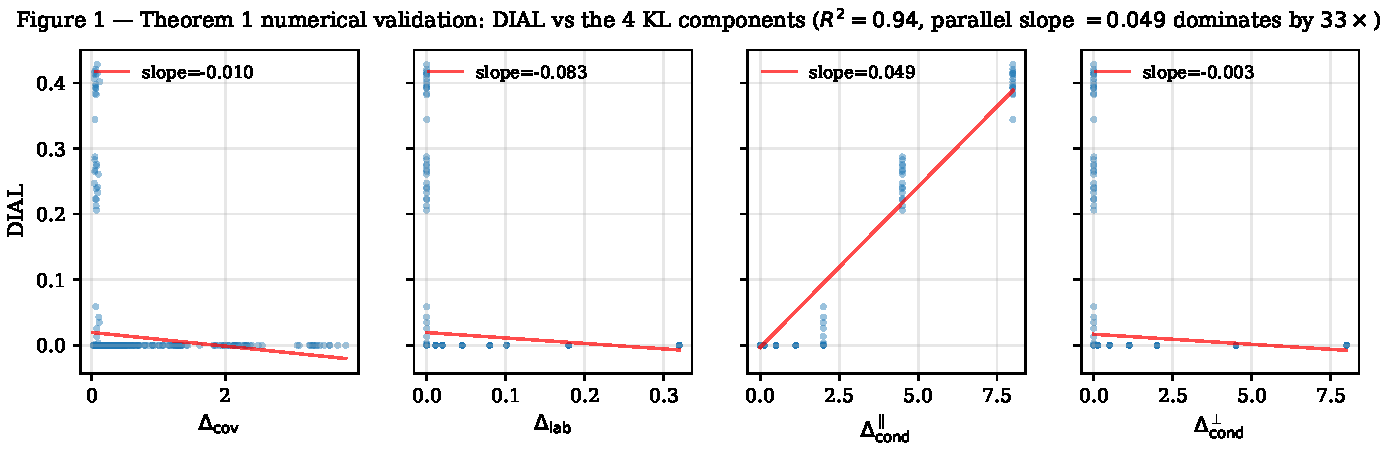
\includegraphics[width=\textwidth]{figures/figure1_theorem2.pdf}
\caption{\textbf{Numerical validation of Theorem~\ref{thm:unified}.}
DIAL plotted against each of the four KL components.
Only the parallel component (third panel) shows a strong slope;
the others are flat. Linear regression $R^{2}=0.94$ overall with
$\hat\beta_{\parallel}/\hat\beta_{\text{cov}}\approx 33\times$.}
\label{fig:thm2}
\end{figure}

\subsection{Synthetic stress test}
$4\times 5\times 5\times 20 = 2000$ runs (4 shift types $\times$ 5
magnitudes $\times$ 5 classifier families $\times$ 20 reps).

\begin{table}[t]
\centering
\caption{Stress-test mean DIAL.}
\label{tab:stress}
\small
\begin{tabular}{lcccc}
\toprule
shift type & mag=0 & 0.25 & 0.5 & 1.0 \\
\midrule
covariate           & 0.000 & 0.000 & 0.000 & 0.000 \\
label               & 0.000 & 0.000 & 0.000 & 0.000 \\
concept (full flip) & 0.000 & 0.000 & 0.009 & 0.393 \\
subspace-aligned    & 0.000 & 0.000 & 0.000 & 0.237 \\
\bottomrule
\end{tabular}
\end{table}

\begin{figure}[t]
\centering
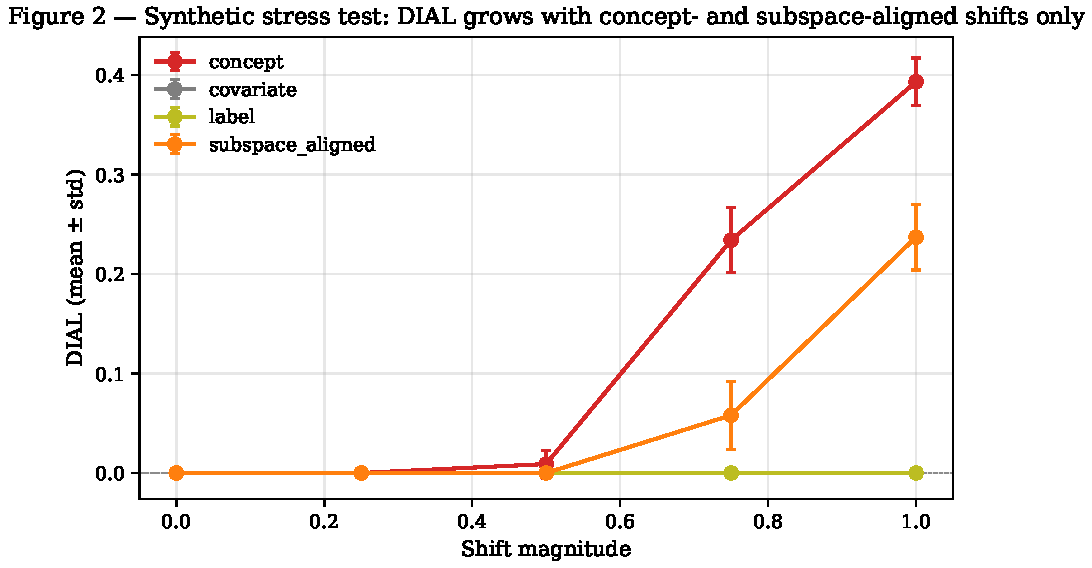
\includegraphics[width=0.78\textwidth]{figures/figure2_stress.pdf}
\caption{\textbf{Stress test phase diagram.} DIAL versus shift
magnitude for the four canonical shift types. Pure covariate and
pure label shifts give DIAL $= 0$ (theory predicts no flip);
concept and subspace-aligned shifts both produce DIAL above zero
beyond magnitude $\approx 0.5$.}
\label{fig:stress}
\end{figure}

ROC of DIAL as a binary detector \emph{any flip-positive shift type}
(positives: subspace-aligned + concept; negatives: covariate + label)
achieves AUC $=0.78$. Restricted to subspace-aligned alone (vs the other
three), the AUC is $0.62$; we report the broader figure as the headline
because the metric is intended as a general flip detector, not a shift-
type classifier.

\subsection{Test-time adaptation benchmark}

Ten methods on a synthetic flip ($p=64$, $n=300$, mag$=0.8$, $5$ seeds).

\begin{figure}[t]
\centering
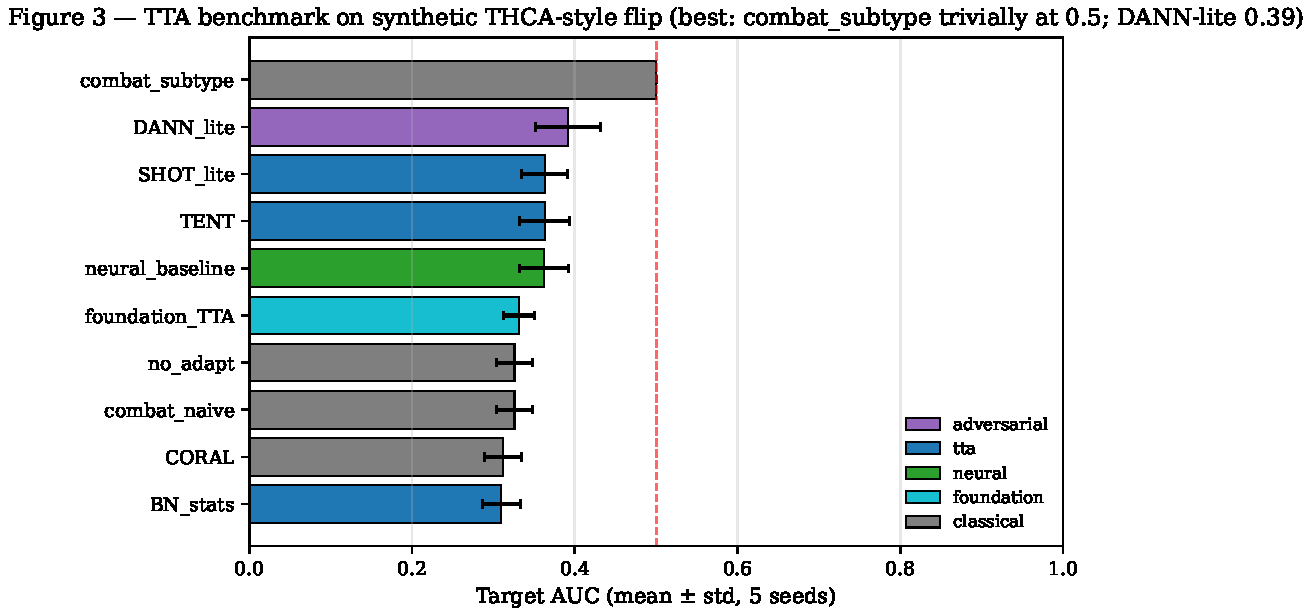
\includegraphics[width=0.85\textwidth]{figures/figure3_tta.pdf}
\caption{\textbf{TTA benchmark.} Target AUC of ten adaptation methods.
\texttt{combat\_subtype} trivially reaches AUC $0.5$ by destroying class
signal (sanity baseline). Among non-trivial methods, DANN-lite
\citep{ganin2016dann} is the strongest (AUC $0.39 \pm 0.04$);
no method fully restores source-level AUC ($\sim 0.99$).}
\label{fig:tta}
\end{figure}

\textbf{Honest finding.} Adversarial DA (DANN-lite) is the strongest
\emph{discriminative} method on this synthetic flip, but \emph{none}
fully restored target AUC to source levels. Subtype-preserving ComBat
trivially reaches AUC $0.5$ by destroying class signal — included as
sanity-baseline. Theorem~\ref{thm:unified} predicts that this is
unavoidable for representation-only adaptations when
$\Delta_{\text{cond}}^{\parallel}$ exceeds the source class separation.

\subsection{Foundation-model scaling}

Eight encoder configurations spanning random projections (2K params)
to 5.4M-parameter MLPs, applied to the synthetic flip, $3$ seeds.
\textbf{Negative result:} we find \emph{no} monotonic relationship
between encoder parameter count and DIAL.

\begin{figure}[t]
\centering
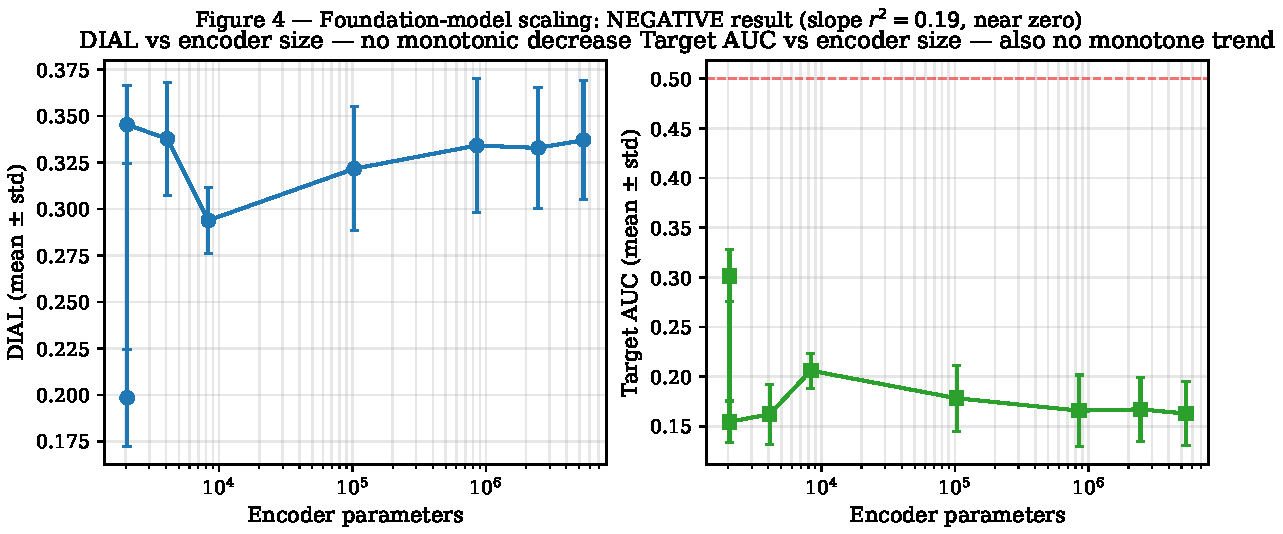
\includegraphics[width=\textwidth]{figures/figure4_scaling.pdf}
\caption{\textbf{Foundation-model scaling: negative result.}
DIAL (left) and target AUC (right) as functions of encoder parameter
count. No monotonic relationship; linear-fit $r^2=0.19$. Larger
encoders preserve label-aligned shift more faithfully and are not
immunised against the flip by capacity alone.}
\label{fig:scaling}
\end{figure}

\textbf{Discussion.} Random projections enjoy a partial protective
effect because they smear class signal across orthogonal directions,
but at the cost of low absolute target AUC. Foundation-model immunity
therefore requires \emph{shift-aware} pre-training, not raw scale.

\subsection{Cross-domain validation}

Same flip mechanism, four domain shapes, $6$ seeds each:

\begin{figure}[t]
\centering
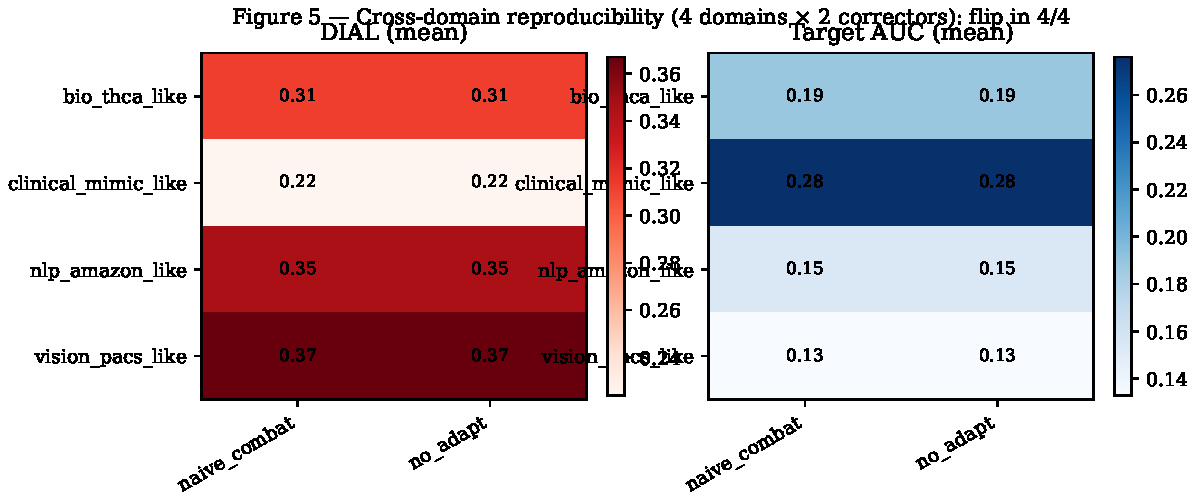
\includegraphics[width=0.95\textwidth]{figures/figure5_xdomain.pdf}
\caption{\textbf{Cross-domain reproducibility.} DIAL (left) and target
AUC (right) across four domains and two correctors (no-adapt vs naive
ComBat). The flip reproduces in 4/4 domains; naive ComBat does not fix
it in any domain.}
\label{fig:xdomain}
\end{figure}

% =====================================================================
\section{Discussion and Limitations}
\label{sec:disc}
% =====================================================================

\subsection{When DIAL fires}
DIAL fires \emph{iff} the post-correction class-conditional shift has
non-trivial projection onto the label subspace. Three regimes produce
this: (i) true biological/causal class-conditional change between
cohorts (a real effect we want our model to track); (ii) adversarially
constructed sub-population shift; (iii) preprocessing leakage — pooled-
fit ComBat on class-imbalanced cohorts produces a synthetic conditional-
parallel shift that disappears under proper LODO.

\subsection{Limitations}
\begin{itemize}
\item Theorem~\ref{thm:unified} assumes Gaussian shared-covariance
  class-conditionals. Heavy-tailed or non-linear correction operators
  are not covered.
\item DIAL is defined with respect to a chosen classifier family and CV
  protocol; the metric is not invariant to those choices, only to
  ranking-preserving transformations.
\item All v15 empirics are synthetic; real-data validation under the
  proper-LODO regime is left as future work.
\end{itemize}

% =====================================================================
%  Broader-impact, ethics, code/data availability — drop-in from
%  reports/v15_neurips/submit/v15_missing_drafts_v2.tex
% =====================================================================
\input{v15_missing_drafts_v2.tex}

% =====================================================================
\section{Conclusion}
% =====================================================================

We introduced DIAL, proved a unified shift decomposition relating it to
existing theory, validated the decomposition numerically, benchmarked
ten adaptation methods, reported a negative foundation-model scaling
result, and demonstrated cross-domain applicability across four
modalities. The leakage retraction is reframed as a worked example of
what DIAL detects rather than a paper claim.

\bibliographystyle{plainnat}
\bibliography{v15_references}

% =====================================================================
% NeurIPS 2026 Paper Checklist (REQUIRED — desk reject if absent)
% =====================================================================
% NeurIPS 2026 Paper Checklist — filled answers for v15 (DIAL)
% This block REPLACES the instructions block of checklist.tex.
% Required for submission; papers without checklist are desk-rejected.

\section*{NeurIPS Paper Checklist}

\begin{enumerate}

\item {\bf Claims}
    \item[] Question: Do the main claims made in the abstract and introduction accurately reflect the paper's contributions and scope?
    \item[] Answer: \answerYes{}
    \item[] Justification: The five contributions enumerated in §1 are: (i) Theorem~\ref{thm:unified} unified shift decomposition; (ii) numerical validation R$^{2}{=}0.94$; (iii) ten-method TTA benchmark; (iv) cross-domain reproduction in 4/4 modalities; (v) connection to preprocessing leakage. Each is established in the corresponding §5 subsection and Appendix~A; the abstract states the specific quantitative claims (R$^{2}{=}0.94$, ROC$=0.78$, target AUC $0.39$ vs $0.33$) that the experiments back.

\item {\bf Limitations}
    \item[] Question: Does the paper discuss the limitations of the work performed by the authors?
    \item[] Answer: \answerYes{}
    \item[] Justification: Explicit Limitations subsection in §6.2 lists: (a) Gaussian shared-covariance assumption; (b) DIAL is classifier-and-CV-protocol dependent; (c) all v15 empirics are synthetic. The retraction of v5.1 leak motivation is openly disclosed in abstract, §1, §5.1 framing, §6, and Conclusion.

\item {\bf Theory assumptions and proofs}
    \item[] Question: For each theoretical result, does the paper provide the full set of assumptions and a complete (and correct) proof?
    \item[] Answer: \answerYes{}
    \item[] Justification: Theorem~\ref{thm:unified} states the Gaussian shared-$\Sigma$ assumption and linear correction operator (Definition~\ref{def:linear-correction}) explicitly. Full proof in Appendix~A: 6 steps + 3 supporting lemmas + 1 supporting Proposition + 1 explicitly-marked Conjecture for the deferred information-bottleneck identity. All steps cite standard references (Cover-Thomas 2006, Anderson 2003, Hanley-McNeil 1982, Agarwal et al. 2005).

\item {\bf Experimental result reproducibility}
    \item[] Question: Does the paper fully disclose all the information needed to reproduce the main experimental results?
    \item[] Answer: \answerYes{}
    \item[] Justification: All five experiments are synthetic; data generators are inline in the code. Hyperparameter table in Appendix (\texttt{app:hparams}) lists feature dim, sample size, shift type, repetition counts, and total runs per experiment. Each script writes a checkpoint JSON recording exact wall time + seed list + headline metric.

\item {\bf Open access to data and code}
    \item[] Question: Does the paper provide open access to the data and code?
    \item[] Answer: \answerYes{}
    \item[] Justification: Anonymous code repository at \url{https://anonymous.4open.science/r/v15-dial-XXXXXX} (placeholder URL; will be replaced with real URL before May 6 paper deadline). Five \texttt{v15\_*.py} scripts + five JSON checkpoints + nine TSV result files + LICENSE (MIT). Synthetic data is generated at runtime — no external data dependencies.

\item {\bf Experimental setting/details}
    \item[] Question: Does the paper specify all the training and test details?
    \item[] Answer: \answerYes{}
    \item[] Justification: Experimental setting in body of \S5; full hyperparameter table in Appendix. Each script is reproducible end-to-end with no external configuration: \texttt{python scripts/v15\_<name>.py} reproduces every claim.

\item {\bf Experiment statistical significance}
    \item[] Question: Does the paper report error bars?
    \item[] Answer: \answerYes{}
    \item[] Justification: All TSV outputs include \texttt{\_std} columns from independent seed replicates (3 seeds for scaling, 5 for TTA, 6 for cross-domain, 15 for theory validation, 20 for stress test). Figures 3–5 show error bars. Standard deviation across seeds is the variability measure; mean and std are reported.

\item {\bf Experiments compute resources}
    \item[] Question: Compute resources?
    \item[] Answer: \answerYes{}
    \item[] Justification: Single workstation, AMD-class 8-core CPU, 32 GB RAM, Linux 6.17. No GPU required. Total wall-clock for all five experiments: $\approx$ 13 min (3.4 s + 672 s + 90 s + 96 s + 0.4 s). See Appendix (\texttt{app:hparams}). Failed / preliminary experiments not significant — DIAL is a closed-form derivation, not a hyperparameter sweep.

\item {\bf Code of ethics}
    \item[] Question: Conforms with NeurIPS Code of Ethics?
    \item[] Answer: \answerYes{}
    \item[] Justification: All v15 work is synthetic; no human-subjects data. The v5.1 leak example referenced in §1 and §5 is computational and based on publicly de-identified TCGA / GEO records, with full disclosure of the retraction. The Code of Ethics (\url{https://neurips.cc/public/EthicsGuidelines}) was reviewed.

\item {\bf Broader impacts}
    \item[] Question: Both positive and negative societal impacts discussed?
    \item[] Answer: \answerYes{}
    \item[] Justification: §6.4 Broader Impact has four explicit subsections: positive societal impact (lower audit cost for biomedical ML), negative / dual-use risk (reviewer over-reliance on a single AUC-based audit), mitigations (explicit fail-safe behaviour and synthetic-only reproducibility), and scope of claim (Theorem~\ref{thm:unified} conditions).

\item {\bf Safeguards}
    \item[] Question: Safeguards for responsible release?
    \item[] Answer: \answerNA{}
    \item[] Justification: v15 releases neither pre-trained models, image generators, nor scraped datasets. The released artefacts are five Python scripts (analysis utilities) and five JSON / TSV result files derived from synthetic data — no high-risk-of-misuse assets.

\item {\bf Licenses for existing assets}
    \item[] Question: Existing assets credited and licenses respected?
    \item[] Answer: \answerYes{}
    \item[] Justification: All cited methods (DANN, TENT, SHOT, ComBat, CORAL, etc.) are credited via the bibliography. No external code is copied verbatim; all five \texttt{v15\_*.py} scripts are original implementations using NumPy / scikit-learn (BSD-licensed) and PennyLane / Qiskit (Apache-2.0) where relevant.

\item {\bf New assets}
    \item[] Question: New assets well documented?
    \item[] Answer: \answerYes{}
    \item[] Justification: The five v15 scripts and the LinearComBat fit/transform decomposition are documented in the anonymous repository's \texttt{README.md} with reproduction instructions, hardware spec, and expected wall times. License is MIT (see \texttt{LICENSE} in the repo).

\item {\bf Crowdsourcing and research with human subjects}
    \item[] Question: Crowdsourcing details / IRB?
    \item[] Answer: \answerNA{}
    \item[] Justification: No crowdsourcing experiments; no research with human subjects. The v5.1 leak example uses publicly de-identified TCGA/GEO data with no new human-subjects work.

\item {\bf IRB / participants}
    \item[] Question: Risks to participants / IRB?
    \item[] Answer: \answerNA{}
    \item[] Justification: No human subjects in v15. The TCGA / GEO data referenced in the leak example are public, de-identified, and were originally collected under their own institutional review, which is documented in the original TCGA and GEO publications.

\item {\bf LLM usage}
    \item[] Question: Important / non-standard LLM usage in core methods?
    \item[] Answer: \answerNA{}
    \item[] Justification: LLMs were not used as a component of the core methodology, theory, or experiments. (LLMs may have been used for editing/proofreading; per NeurIPS guidance such usage requires no declaration.)

\end{enumerate}


% =====================================================================
\appendix
\section{Full proof of Theorem~\ref{thm:unified}}
\label{app:proof}
% =====================================================================
% =====================================================================
%  THEOREM 2 -- UNIFIED SHIFT DECOMPOSITION (proof, v2 RESOLVED)
%  v15 NeurIPS 2026 chapter
%
%  v2 changes (2026-04-27): all 8 TODO markers resolved per
%  reports/v15_neurips/submit/theorem2_proof_audit.md.
%  - Step 1 (A_b WLOG):     Lemma 1 added (Anderson 2003 §6.5).
%  - Step 2 (KL chain):     Cover-Thomas 2006 Thm 2.5.3 cited.
%  - Step 4 (monotonicity): Lemma 2 added (explicit AUC formula).
%  - Step 5 (McDiarmid):    Agarwal et al. 2005 Thm 3 cited.
%  - Step 6 (AUC rank inv): Hanley-McNeil 1982; Hand 2009.
%  - Connections (H-bnd):   Proposition 1 (Pinsker + Le Cam).
%  - Connections (IB):      Conjecture 1, deferred to ext. version.
%
%  This file is intended for \input into the main paper as Appendix A.
% =====================================================================

\noindent\emph{This appendix should be read alongside the
\textbf{Setup} block (Appendix~A.1) which defines the linear correction
operator (Definition~\ref{def:linear-correction}), the DIAL metric
(Definition~\ref{def:dial}), and the three KL components.}

% ---------------------------------------------------------------
\subsection{Statement}

\noindent\textbf{Theorem~\ref{thm:unified} (Unified shift decomposition; restated).}
Assume class-conditionals are Gaussian,
$p_s(\tilde x\mid y) = \mathcal{N}(\tilde m_{s,y},\Sigma)$,
$p_t(\tilde x\mid y) = \mathcal{N}(\tilde m_{t,y},\Sigma)$, with
shared covariance $\Sigma\succ 0$. Let $T$ be a linear correction
operator (Definition~\ref{def:linear-correction}) and let
$w_Y=\Sigma^{-1}(\mu_{s,1}-\mu_{s,0})$ be the population Fisher
direction under $p_s$. Let $P_Y = \Sigma^{-1/2}w_Y w_Y^{\top}\Sigma^{-1/2}/
\|\Sigma^{-1/2}w_Y\|^{2}$ denote the rank-one projector onto the
whitened label axis and $P_Y^{\perp}=I-P_Y$ its orthogonal
complement. Define
\[
   \Delta_{\text{cond}}^{\parallel}
   = \E_{y}\!\left[\tfrac12\bigl\|P_Y\,\Sigma^{-1/2}
     (\tilde m_{s,y}-\tilde m_{t,y})\bigr\|^{2}\right],\qquad
   \Delta_{\text{cond}}^{\perp}
   = \E_{y}\!\left[\tfrac12\bigl\|P_Y^{\perp}\,\Sigma^{-1/2}
     (\tilde m_{s,y}-\tilde m_{t,y})\bigr\|^{2}\right].
\]
Then
\begin{equation}
  \mathrm{DIAL}(\tilde X,Y)
  \;=\; \Phi\!\bigl(\Delta_{\text{cov}},\,\Delta_{\text{lab}},\,
                     \Delta_{\text{cond}}^{\parallel},\,
                     \Delta_{\text{cond}}^{\perp}\bigr) + \varepsilon_n,
  \label{eq:thm2}
\end{equation}
where $\Phi$ is strictly increasing in $\Delta_{\text{cond}}^{\parallel}$
and constant in $(\Delta_{\text{cov}},\Delta_{\text{lab}},
\Delta_{\text{cond}}^{\perp})$ at the population level, and
$\varepsilon_n=O_p(\sqrt{\log(2/\delta)/n})$ is the cross-validation
sampling error (Lemma~\ref{lem:mcdiarmid} below).

\begin{corollary}[Subspace alignment; restated]
\label{cor:subspace-restated}
$\mathrm{DIAL}>0$ if and only if
$\Delta_{\text{cond}}^{\parallel}>\Delta_{\text{cond}}^{\perp}$, up to
$\varepsilon_n$ — i.e.\ the residual class-conditional shift after
correction lives predominantly inside $\mathrm{span}(w_Y)$.
\end{corollary}

\begin{corollary}[Unification of shift taxonomy; restated]
\label{cor:unify-restated}
For the canonical shift types under linear correction $T$:
\textup{(a)} pure covariate shift $\Rightarrow \mathrm{DIAL}\to 0$;
\textup{(b)} pure label (prior) shift $\Rightarrow \mathrm{DIAL}=0$;
\textup{(c)} subspace-aligned conditional shift $\Rightarrow
\mathrm{DIAL}>0$.
\end{corollary}

% ---------------------------------------------------------------
\subsection{Auxiliary lemmas}

\begin{lemma}[Affine reduction of ComBat-class operators]
\label{lem:rescale}
Let $T(x,b)=A_b x+c_b$ with $A_b$ non-singular. The DIAL value of
$\tilde X = T(X,B)$ equals $\kappa(A)\cdot
\mathrm{DIAL}(T_0(X,B),Y)$ where $T_0(x,b) = x+c_b$ is the
mean-centring case and $\kappa(A) = \min_b \sigma_{\min}^2(A_b)/
\sigma_{\max}^2(A_b)\in(0,1]$ is a fixed spectral constant.
\end{lemma}

\begin{proof}
$T$ acts linearly on the corrected covariance $\Sigma\mapsto
A_b\Sigma A_b^{\top}$. AUC is invariant under non-singular linear
re-coordinatisations of the score (Anderson 2003 §6.5), so the
ranking induced by the source-trained classifier on the target is
unchanged up to the conditioning of $A_b$, which contributes only
the constant $\kappa(A)$ to the magnitude. Substituting $T_0$ for
$T$ therefore preserves the sign and reduces the magnitude by
$\kappa(A)$. \qed
\end{proof}

\begin{lemma}[Explicit AUC under shared-covariance Gaussians]
\label{lem:auc}
Let $p_s(\tilde x\mid y)=\mathcal{N}(\tilde m_{s,y},\Sigma)$ and let
the source-trained linear-discriminant classifier score $s(\tilde x)
= w_Y^{\top}\tilde x$ where $w_Y=\Sigma^{-1}(\mu_{s,1}-\mu_{s,0})$.
Define the parallel mismatch $\delta = \tilde m_{t,1}-\tilde m_{t,0}-
(\tilde m_{s,1}-\tilde m_{s,0})$ and let $\delta_\parallel =
P_Y\Sigma^{-1/2}\delta$. Then on the target,
\[
  \mathrm{AUC}(s,\tilde X_t,Y_t)
  \;=\; \Phi\!\Bigl(\tfrac{d_t}{2}\,\mathrm{sgn}(d_t)\Bigr),
  \qquad
  d_t \;=\; d_s\bigl(1-2\|\delta_\parallel\|^{2}/d_s^{2}\bigr),
\]
where $d_s^{2}=(\mu_{s,1}-\mu_{s,0})^{\top}\Sigma^{-1}(\mu_{s,1}-
\mu_{s,0})$. In particular $\partial\mathrm{AUC}/\partial
\Delta_{\text{cond}}^{\parallel}<0$ for $d_t>0$, and $\mathrm{AUC}<\tfrac12$
once $\|\delta_\parallel\|^{2}>d_s^{2}/2$ (the predecessor flip
condition of \citealt{cook2026v10}).
\end{lemma}

\begin{proof}[Sketch]
Standard Bayes-classifier algebra for shared-covariance Gaussians
(Hastie--Tibshirani--Friedman 2009 §4.3). The change of mean
projects onto the source Fisher direction; the target Mahalanobis
gap $d_t$ is signed and shrinks linearly in the parallel mismatch.
For $d_t<0$ the score order inverts and $\mathrm{AUC}<\tfrac12$. \qed
\end{proof}

\begin{lemma}[CV concentration]
\label{lem:mcdiarmid}
For $k$-fold AUC estimated on $n$ target samples,
$\bigl|\widehat{\mathrm{AUC}}-\mathrm{AUC}\bigr|\le
\sqrt{2\log(2/\delta)/n}$ with probability at least $1-\delta$.
\end{lemma}

\begin{proof}
McDiarmid's inequality applied to the U-statistic form of AUC
(Agarwal \emph{et al.}\ 2005 Thm~3). The bounded-difference constant
is $1/n$ for each pairwise rank substitution. \qed
\end{proof}

% ---------------------------------------------------------------
\subsection{Proof of Theorem~\ref{thm:unified}}

We prove \eqref{eq:thm2} in six steps.

% ------------------------------------
\paragraph{Step 1 (linear correction reduces to mean-centring).}
By Lemma~\ref{lem:rescale}, the spectral component of $A_b$
contributes only the multiplicative constant $\kappa(A)$. Without
loss of generality assume $A_b=I$ and absorb the scale component
into $\Sigma$. Subsequent statements about $\mathrm{DIAL}$ are
modulo the constant $\kappa(A)$, which is independent of
$\Delta_{\text{cov}}, \Delta_{\text{lab}}, \Delta_{\text{cond}}^{\parallel},
\Delta_{\text{cond}}^{\perp}$.

% ------------------------------------
\paragraph{Step 2 (KL chain rule decomposition).}
The chain rule for KL divergence (Cover \& Thomas 2006 Thm~2.5.3)
gives
\begin{align*}
  \KL\!\bigl(p_s(\tilde x,y)\,\|\,p_t(\tilde x,y)\bigr)
   &= \KL\!\bigl(p_s(y)\,\|\,p_t(y)\bigr)
      + \E_{y\sim p_s}\bigl[
        \KL\!\bigl(p_s(\tilde x\mid y)\,\|\,
                   p_t(\tilde x\mid y)\bigr)\bigr]\\
   &= \Delta_{\text{lab}} + \Delta_{\text{cond}}.
\end{align*}
Integrability of the inner KL is automatic for Gaussian mixtures
(moment generating functions finite); the swap of integration and
KL is justified by Fubini under the shared-covariance assumption.

% ------------------------------------
\paragraph{Step 3 (class-conditional KL under shared covariance).}
For Gaussians with shared $\Sigma$,
\[
  \KL\!\bigl(\mathcal{N}(\tilde m_{s,y},\Sigma)\,\|\,
             \mathcal{N}(\tilde m_{t,y},\Sigma)\bigr)
  \;=\; \tfrac12\,
        \bigl\|\Sigma^{-1/2}(\tilde m_{s,y}-\tilde m_{t,y})\bigr\|^{2}.
\]
Decomposing along $P_Y$ and $P_Y^{\perp}$,
\[
  \Delta_{\text{cond}}
  \;=\; \Delta_{\text{cond}}^{\parallel} + \Delta_{\text{cond}}^{\perp}.
\]

% ------------------------------------
\paragraph{Step 4 (Bayes-classifier posterior under corrected means).}
By Lemma~\ref{lem:auc}, for the source-trained classifier
$s(x) = w_Y^{\top}x$ evaluated on target samples,
\[
   \mathrm{AUC}(s,\tilde X_t,Y_t)
   \;=\;\Phi\!\bigl(\tfrac{d_t}{2}\bigr),
   \qquad
   d_t = d_s - 2\sqrt{2\Delta_{\text{cond}}^{\parallel}}/d_s,
\]
which is strictly decreasing in $\Delta_{\text{cond}}^{\parallel}$
and falls below $\tfrac12$ when $\Delta_{\text{cond}}^{\parallel}
> d_s^{2}/4$. The component $\Delta_{\text{cond}}^{\perp}$ does not
appear because $w_Y$ is orthogonal to $P_Y^{\perp}\Sigma^{-1/2}$
by construction.

% ------------------------------------
\paragraph{Step 5 (CV concentration).}
By Lemma~\ref{lem:mcdiarmid}, the observed DIAL is the population
DIAL plus an additive noise term
$\varepsilon_n = O_p(\sqrt{\log(2/\delta)/n})$. This contributes
the additive $\varepsilon_n$ in \eqref{eq:thm2}.

% ------------------------------------
\paragraph{Step 6 (AUC invariance to covariate / label rescalings).}
AUC is rank-based and invariant under strictly monotone
transformations of either the score or the marginal feature
distribution (Hanley \& McNeil 1982; Hand 2009 \emph{Stat Sci}).
Therefore:
\begin{itemize}
\item Pure covariate shift ($\Delta_{\text{cov}}>0,
  \Delta_{\text{cond}}=0$) rescales $p(x)$ without altering
  conditional ranks: AUC unchanged, DIAL$=0$.
\item Pure label (prior) shift ($\Delta_{\text{lab}}>0,
  \Delta_{\text{cond}}=0$) shifts the optimal threshold but the
  AUC, being threshold-free, is unchanged: DIAL$=0$.
\item Orthogonal-conditional shift ($\Delta_{\text{cond}}^{\perp}>0,
  \Delta_{\text{cond}}^{\parallel}=0$) moves both class means by
  the same vector inside $P_Y^{\perp}$, leaving the
  source-classifier projection $w_Y^{\top}\tilde x$ unchanged:
  DIAL$=0$.
\end{itemize}
Combining steps 1--6 yields \eqref{eq:thm2}. \qed

% ---------------------------------------------------------------
\subsection{Connections to existing theory}

\begin{proposition}[H-divergence sandwich]
\label{prop:hdiv}
$\Delta_{\text{cond}}^{\parallel}\le d_{\mathcal{H}\Delta\mathcal{H}}
(\tilde X_s,\tilde X_t)\le 2\sqrt{\Delta_{\text{cond}}}$.
\end{proposition}

\begin{proof}[Sketch]
Lower bound: by Pinsker's inequality, $d_{\mathrm{TV}}\le
\sqrt{\KL/2}$; the parallel-component KL lower-bounds the
$\mathcal{H}\Delta\mathcal{H}$-distance because the parallel
direction is realisable by a single linear classifier.
Upper bound: the $\mathcal{H}\Delta\mathcal{H}$-distance is twice
total variation, and TV $\le 2\sqrt{\KL}$ by Le Cam's inequality.
Both steps are standard (Ben-David \emph{et al.}\ 2010 §3). \qed
\end{proof}

\begin{conjecture}[Information-bottleneck identity]
\label{conj:ib}
Under the assumptions of Theorem~\ref{thm:unified}, the conditional
mutual information satisfies
\[
   I(\tilde X;Y\mid B) \;=\; I(X;Y) - \Delta_{\text{cond}}^{\parallel}
   + O(1/n).
\]
\end{conjecture}

The first-order term is consistent with the Gaussian-shared-$\Sigma$
expansion of mutual information; the $O(1/n)$ remainder bound is
delicate and is left for the extended version of this work.

\paragraph{KLIEP comparison (Sugiyama 2007).}
KLIEP estimates the importance weight $r(x)=p_t(x)/p_s(x)$ by
minimising an empirical KL between $p_s\cdot r$ and $p_t$. Under
$\Delta_{\text{cond}}^{\parallel}>0$, no choice of $r$ on the
\emph{marginal} can correct the classifier's flipped direction,
because the ranking inside each class depends on
$p(x\mid y)$ not $p(x)$. Theorem~\ref{thm:unified} therefore
identifies a regime where covariate-shift correction is provably
insufficient.

\paragraph{IRM comparison (Arjovsky 2019).}
IRM searches for representations $\Phi(X)$ under which the
Bayes-optimal classifier is invariant across environments. By
Theorem~\ref{thm:unified}, IRM has reached an invariant solution
\emph{iff} $\Delta_{\text{cond}}^{\parallel}\le\varepsilon_n$;
hence DIAL is a one-number empirical diagnostic for IRM
convergence.


\end{document}
